\documentclass[journal,12pt,twocolumn]{IEEEtran}

 \usepackage{setspace}
 \usepackage{gensymb}
 \usepackage{graphicx}

 \singlespacing

\graphicspath{ {/user/adarshsrivastava/desktop/Matrix Theory/Assignemnt_5} }
 \usepackage[cmex10]{amsmath}

 \usepackage{amsthm}
 \usepackage{hyperref}
 \usepackage{mathrsfs}
 \usepackage{txfonts}
 \usepackage{stfloats}
 \usepackage{bm}
 \usepackage{cite}
 \usepackage{cases}
 \usepackage{subfig}

 \usepackage{longtable}
 \usepackage{multirow}

 \usepackage{enumitem}
 \usepackage{mathtools}
 \usepackage{steinmetz}
 \usepackage{tikz}
 \usepackage{circuitikz}
 \usepackage{verbatim}
 \usepackage{tfrupee}
 \usepackage[breaklinks=true]{hyperref}

 \usepackage{tkz-euclide}

 \usetikzlibrary{calc,math}
 \usepackage{listings}
     \usepackage{color}                                            %%
     \usepackage{array}                                            %%
     \usepackage{longtable}                                        %%
     \usepackage{calc}                                             %%
     \usepackage{multirow}                                         %%
     \usepackage{hhline}                                           %%
     \usepackage{ifthen}                                           %%
     \usepackage{lscape}     
 \usepackage{multicol}
 \usepackage{chngcntr}

 \DeclareMathOperator*{\Res}{Res}

 \renewcommand\thesection{\arabic{section}}
 \renewcommand\thesubsection{\thesection.\arabic{subsection}}
 \renewcommand\thesubsubsection{\thesubsection.\arabic{subsubsection}}

 \renewcommand\thesectiondis{\arabic{section}}
 \renewcommand\thesubsectiondis{\thesectiondis.\arabic{subsection}}
 \renewcommand\thesubsubsectiondis{\thesubsectiondis.\arabic{subsubsection}}


 \hyphenation{op-tical net-works semi-conduc-tor}
 \def\inputGnumericTable{}                                 %%

 \lstset{
 %language=C,
 frame=single, 
 breaklines=true,
 columns=fullflexible
 }
 \begin{document}


 \newtheorem{theorem}{Theorem}[section]
 \newtheorem{problem}{Problem}
 \newtheorem{proposition}{Proposition}[section]
 \newtheorem{lemma}{Lemma}[section]
 \newtheorem{corollary}[theorem]{Corollary}
 \newtheorem{example}{Example}[section]
 \newtheorem{definition}[problem]{Definition}

 \newcommand{\BEQA}{\begin{eqnarray}}
 \newcommand{\EEQA}{\end{eqnarray}}
 \newcommand{\define}{\stackrel{\triangle}{=}}
 \bibliographystyle{IEEEtran}
 \providecommand{\mbf}{\mathbf}
 \providecommand{\pr}[1]{\ensuremath{\Pr\left(#1\right)}}
 \providecommand{\qfunc}[1]{\ensuremath{Q\left(#1\right)}}
 \providecommand{\sbrak}[1]{\ensuremath{{}\left[#1\right]}}
 \providecommand{\lsbrak}[1]{\ensuremath{{}\left[#1\right.}}
 \providecommand{\rsbrak}[1]{\ensuremath{{}\left.#1\right]}}
 \providecommand{\brak}[1]{\ensuremath{\left(#1\right)}}
 \providecommand{\lbrak}[1]{\ensuremath{\left(#1\right.}}
 \providecommand{\rbrak}[1]{\ensuremath{\left.#1\right)}}
 \providecommand{\cbrak}[1]{\ensuremath{\left\{#1\right\}}}
 \providecommand{\lcbrak}[1]{\ensuremath{\left\{#1\right.}}
 \providecommand{\rcbrak}[1]{\ensuremath{\left.#1\right\}}}
 \theoremstyle{remark}
 \newtheorem{rem}{Remark}
 \newcommand{\sgn}{\mathop{\mathrm{sgn}}}
 \providecommand{\abs}[1]{\left\vert#1\right\vert}
 \providecommand{\res}[1]{\Res\displaylimits_{#1}} 
 \providecommand{\norm}[1]{\left\lVert#1\right\rVert}
 %\providecommand{\norm}[1]{\lVert#1\rVert}
 \providecommand{\mtx}[1]{\mathbf{#1}}
 \providecommand{\mean}[1]{E\left[ #1 \right]}
 \providecommand{\fourier}{\overset{\mathcal{F}}{ \rightleftharpoons}}
 %\providecommand{\hilbert}{\overset{\mathcal{H}}{ \rightleftharpoons}}
 \providecommand{\system}{\overset{\mathcal{H}}{ \longleftrightarrow}}
 	%\newcommand{\solution}[2]{\textbf{Solution:}{#1}}
 \newcommand{\solution}{\noindent \textbf{Solution: }}
 \newcommand{\cosec}{\,\text{cosec}\,}
 \providecommand{\dec}[2]{\ensuremath{\overset{#1}{\underset{#2}{\gtrless}}}}
 \newcommand{\myvec}[1]{\ensuremath{\begin{pmatrix}#1\end{pmatrix}}}
 \newcommand{\mydet}[1]{\ensuremath{\begin{vmatrix}#1\end{vmatrix}}}
 \numberwithin{equation}{subsection}
 \makeatletter
 \@addtoreset{figure}{problem}
 \makeatother
 \let\StandardTheFigure\thefigure
 \let\vec\mathbf
 \renewcommand{\thefigure}{\theproblem}
 \def\putbox#1#2#3{\makebox[0in][l]{\makebox[#1][l]{}\raisebox{\baselineskip}[0in][0in]{\raisebox{#2}[0in][0in]{#3}}}}
      \def\rightbox#1{\makebox[0in][r]{#1}}
      \def\centbox#1{\makebox[0in]{#1}}
      \def\topbox#1{\raisebox{-\baselineskip}[0in][0in]{#1}}
      \def\midbox#1{\raisebox{-0.5\baselineskip}[0in][0in]{#1}}
 \vspace{3cm}
 \title{Assignment 5}
 \author{Adarsh Srivastava}
 \maketitle
 \newpage
 \bigskip
 %\renewcommand{\thefigure}{\theenumi}
 \renewcommand{\thetable}{\theenumi}
 The link to the solution is
 \begin{lstlisting}
  https://github.com/Adarsh1310/EE5609
 \end{lstlisting}
 \begin{abstract}
 This documents solves a problem based on circles.
 \end{abstract}
 \section{\textbf{Problem}}
Find the area of the region bounded by the circle $\bf{x}^{T}$ $\bf{x}$= 2 and \norm{\vec{x}-\myvec{2\\0}}=2.
 \section{\textbf{Solution}}
 \norm{\vec{x}}^2 + 2\vec{u}^T\vec{x} + f = 0\\
 $So from above equation we can say that,
 \subsection{Circle 1}
 Taking equation of the first circle to be,
 \begin{align}
 \norm{\vec{x}}^2 + 2\vec{u}_1^T\vec{x} + f_1 = 0\\
 {\vec{x}^{T}\vec{x}}-2=0 \text{(given)}\\
 \vec{u_1}=\myvec{0\\0}\\
 \vec{f_1}=-2
 \end{align}
 Hence,radius=$\sqrt{2}$.\\
 \subsection{Circle 2}
Taking equation of the second circle to be,
\begin{align}
\norm{\vec{x}}^2 + 2\vec{u}_2^T\vec{x} + f_2 = 0\\
  \norm{\vec{x}-\myvec{2\\0}}^2 \text{(given)}\\
  {\vec{x}^{T}\vec{x}-2\vec{u}^T\vec{x}}-(\norm{x}+f_2)=0\\
  \vec{u_2}=\myvec{2\\0}\\
 \vec{f_2}=-4
  \end{align}
  Hence,radius=2.\\
 \begin{figure}[h!]
	\centering
	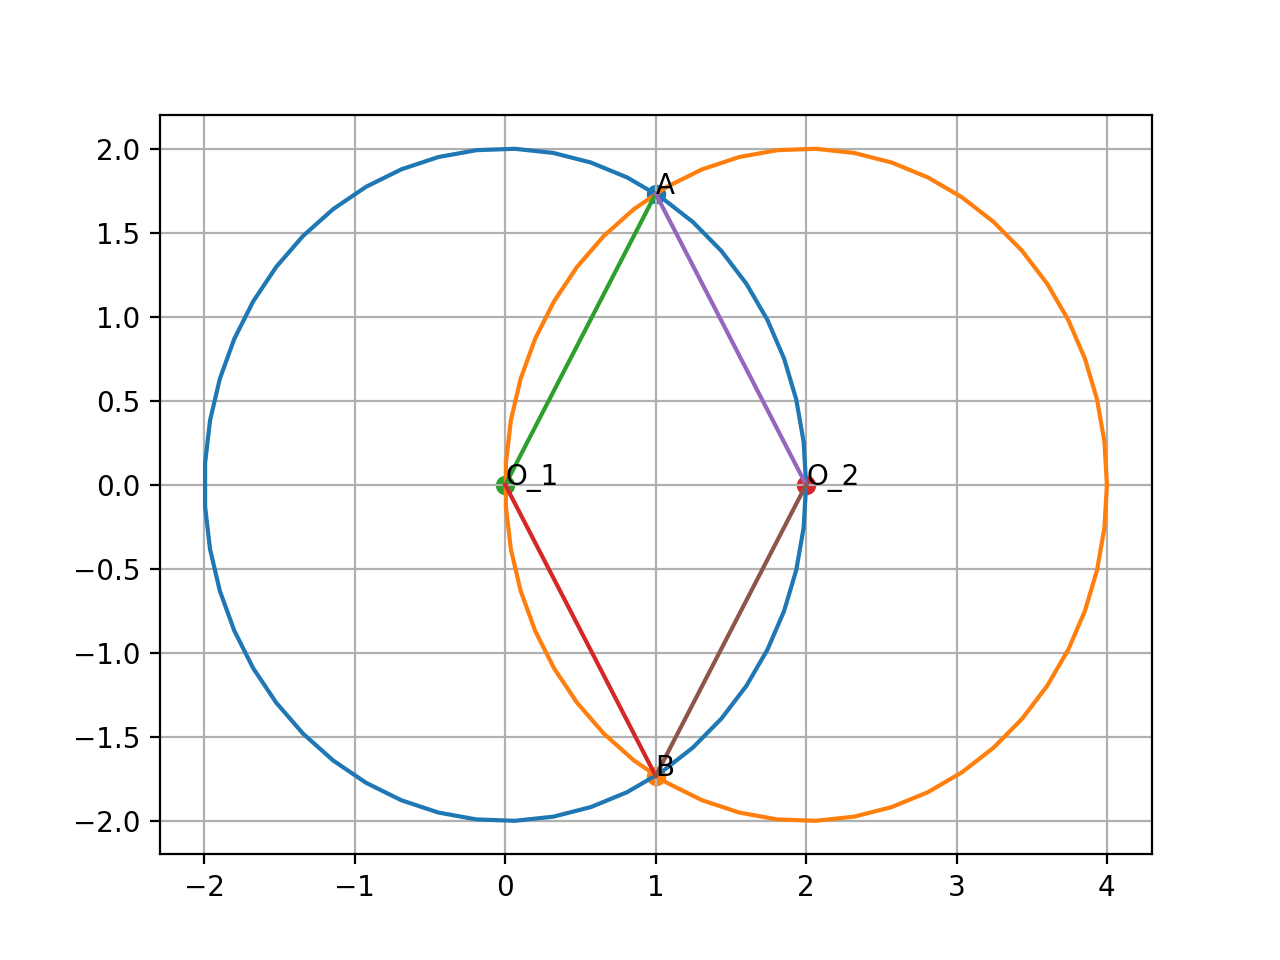
\includegraphics[width=\columnwidth]{Assignment_5.png}
	\caption{Figure depicting intersection points of circle}
	\label{myfig}
\end{figure}
Now,Subtracting equation \eqref{2.2.3} from \eqref{2.1.2} We get,
 \begin{align}
 {\vec{x}^{T}\vec{x}-2\vec{u}^T\vec{x}}-f_1-\bf{x}^{T}\bf{x}-(\norm{x}+f_2)=0\\
 2\vec{u}^{T}\vec{x}=0\\
 \myvec{4&0}\vec{x}=0\text{(Substituting \eqref{} in \eqref{})}
 \end{align}
 Which can be written as:-
 \begin{align}
 \myvec{1&0}\vec{x}=0\\
 \vec{x} = \lambda \vec{m}, \text{where} \vec{m} = \myvec{0\\1}\\
 \vec{x} = \lambda \myvec{0\\1}
 \end{align}
 Substituting \eqref{2.2.9} in \eqref{2.1.2}\\
 \begin{align}
 \lambda\myvec{0\\1}\lambda\myvec{0&1}=2\\
 \lambda=\sqrt{2}
 \end{align}
 Substituting the value of \eqref{} in \eqref{}
 \begin{align}
 \vec{\lambda} = +\sqrt{2}\myvec{0\\1} and - \sqrt{2}\myvec{0\\1}
 \end{align}
 Now to find the area enclosed between these circles we have to find the integral of these point w.r.t the circles.For this we need to find the area of segment  and double it to find the area of the entire overlapped region. To find the area of segment we need angle segment makes.Here,r=$\sqrt{2}$ and $\theta$=angle of segment.Now we have to find the angle.\\ 
\begin{align*}
\sin \theta=\frac{\vec{P}}{\vec{H}}\\ 
\theta=90^{\circ}\\
Total angle=180^{\circ}\\
\end{align*}
 \begin{align}
 \begin{multlined}
 Area=\frac{1}{2}(\frac{180}{360}\pi-\sin (180))r^{2}\\
 $(Area of Sector-Area of Triangle)$
\end{multlined}\\
Area={\frac{1}{2}}(\frac{\pi}{2}-\sin 180)2\\
=2{\frac{1}{2}}(\frac{\pi}{2}-\sin 180)\\
Total area=2*Area\\
=\frac{2\pi-4}{2}
\end{align}

 
  \end{document}